% template.tex, daed April 5 2013
% This is a template file for Annual Reviews 1 column Journals
%
% Compilation using ar-1col.cls' - version 1.0, Aptara Inc.
% (c) 2013 AR
%
% Steps to compile: latex latex latex
%
% For tracking purposes => this is v1.0 - Apr. 2013

\documentclass{ar-1col}\usepackage[]{graphicx}\usepackage[]{color}
% maxwidth is the original width if it is less than linewidth
% otherwise use linewidth (to make sure the graphics do not exceed the margin)
\makeatletter
\def\maxwidth{ %
  \ifdim\Gin@nat@width>\linewidth
    \linewidth
  \else
    \Gin@nat@width
  \fi
}
\makeatother

\definecolor{fgcolor}{rgb}{0.345, 0.345, 0.345}
\makeatletter
\@ifundefined{AddToHook}{}{\AddToHook{package/xcolor/after}{\definecolor{fgcolor}{rgb}{0.345, 0.345, 0.345}}}
\makeatother
\newcommand{\hlnum}[1]{\textcolor[rgb]{0.686,0.059,0.569}{#1}}%
\newcommand{\hlstr}[1]{\textcolor[rgb]{0.192,0.494,0.8}{#1}}%
\newcommand{\hlcom}[1]{\textcolor[rgb]{0.678,0.584,0.686}{\textit{#1}}}%
\newcommand{\hlopt}[1]{\textcolor[rgb]{0,0,0}{#1}}%
\newcommand{\hlstd}[1]{\textcolor[rgb]{0.345,0.345,0.345}{#1}}%
\newcommand{\hlkwa}[1]{\textcolor[rgb]{0.161,0.373,0.58}{\textbf{#1}}}%
\newcommand{\hlkwb}[1]{\textcolor[rgb]{0.69,0.353,0.396}{#1}}%
\newcommand{\hlkwc}[1]{\textcolor[rgb]{0.333,0.667,0.333}{#1}}%
\newcommand{\hlkwd}[1]{\textcolor[rgb]{0.737,0.353,0.396}{\textbf{#1}}}%
\let\hlipl\hlkwb

\usepackage{framed}
\makeatletter
\newenvironment{kframe}{%
 \def\at@end@of@kframe{}%
 \ifinner\ifhmode%
  \def\at@end@of@kframe{\end{minipage}}%
  \begin{minipage}{\columnwidth}%
 \fi\fi%
 \def\FrameCommand##1{\hskip\@totalleftmargin \hskip-\fboxsep
 \colorbox{shadecolor}{##1}\hskip-\fboxsep
     % There is no \\@totalrightmargin, so:
     \hskip-\linewidth \hskip-\@totalleftmargin \hskip\columnwidth}%
 \MakeFramed {\advance\hsize-\width
   \@totalleftmargin\z@ \linewidth\hsize
   \@setminipage}}%
 {\par\unskip\endMakeFramed%
 \at@end@of@kframe}
\makeatother

\definecolor{shadecolor}{rgb}{.97, .97, .97}
\definecolor{messagecolor}{rgb}{0, 0, 0}
\definecolor{warningcolor}{rgb}{1, 0, 1}
\definecolor{errorcolor}{rgb}{1, 0, 0}
\makeatletter
\@ifundefined{AddToHook}{}{\AddToHook{package/xcolor/after}{
\definecolor{shadecolor}{rgb}{.97, .97, .97}
\definecolor{messagecolor}{rgb}{0, 0, 0}
\definecolor{warningcolor}{rgb}{1, 0, 1}
\definecolor{errorcolor}{rgb}{1, 0, 0}
}}
\makeatother
\newenvironment{knitrout}{}{} % an empty environment to be redefined in TeX

\usepackage{alltt}
\usepackage{comment}

\usepackage{tikz}
\usetikzlibrary{trees}

\usepackage{gb4e}
\usepackage{natbib}
\usepackage{url}
\usepackage{amsmath}

%% Make sure that the file is compiled with knitr:
% !Rnw weave = knitr
%% set compiler
% !TeX program = XeLaTeX

\setcounter{secnumdepth}{4}

% Metadata Information
\jname{Annual Reviews of Linguistics}
\jvol{AA}
\jyear{2022}
\doi{10.1146/((please add article doi))}


% Document starts
\IfFileExists{upquote.sty}{\usepackage{upquote}}{}
\begin{document}

% Page header
\markboth{Shravan Vasishth}{Analyzing data}

% Title
\title{Some right ways to analyze (psycho)linguistic data}


%Authors, affiliations address.
\author{Shravan Vasishth$^1$
\affil{$^1$Department of Linguistics, University of Potsdam, Potsdam 14476, Brandenburg, Germany; email: vasishth@uni-potsdam.de; orcid: 0000-0003-2027-1994}}

%Abstract
\begin{abstract}
Much has been written on the abuse and misuse of statistical methods, including p-values, statistical significance, etc. I present some of the best practices in statistics using a running example data analysis. Focusing primarily on frequentist and Bayesian linear mixed models, I illustrate some defensible ways in which statistical inference---specifically, hypothesis testing using Bayes factors vs.\ estimation or uncertainty quantification---can be carried out. The key is to not overstate the evidence and to not expect too much from statistics. Along the way, I demonstrate some powerful ideas, the most important ones being using simulation to understand the design properties of one's experiment before running it, visualizing data before carrying out a formal analysis, and simulating data from the fitted model to understand the model's behavior. 
%I close by pointing out that linguistics can only have a robust empirical base if editors, reviewers, and journals are willing to rethink how empirical research is reported.
\end{abstract}

%Keywords, etc.
\begin{keywords}
Statistics, simulation, experimental science, data analysis, significance testing, Bayesian statistics, Bayes factors, estimation,  uncertainty quantification, transparency, open science
\end{keywords}
\maketitle

%Table of Contents
\tableofcontents



% Heading 1
\section{INTRODUCTION}


\begin{quote}
\textit{If you worked in areas inhabited by demons you would be in trouble regardless of the perfection of your experimental designs.}

\citep[][p. 192]{hurlbert1984pseudoreplication}
\end{quote}

Despite the title of this review, there are no clearly ``right'' ways to analyze data. Statistical data analysis is an inherently subjective process, and it would not be unusual to find that two statisticians analyze the same data very differently and even come to different conclusions/decisions. Yet, both approaches could, at least technically, be correct. Nevertheless, there are some basic principles that come from best practice in statistics that can improve the quality of our statistical inferences. Every sub-field has its own particular sets of commonly used statistical models; in linguistics, the modern standard is the linear mixed model, also referred to as the hierarchical model \citep{pinheirobates}.  Accordingly, in this review, I will focus on this modeling framework. I will discuss both frequentist and Bayesian versions of the hierarchical model.

In what follows, I assume that the reader has a basic knowledge of the t-test and Type I and II errors, and has some experience with the linear mixed model \citep{lme4new}. If the reader lacks this background,  introductory articles like \citet{baayen2008mixed,VasishthNicenboimStatMeth,VasishthBeckmanetal} would be a good starting point. Other, more comprehensive textbook references are provided at the end of this article.


Experimental science is more than careful experiment designs and the use of sophisticated methods like ERPs and eye-tracking. There are six components in an experiment: (i) setting up a research hypothesis, (ii) designing the experiment, (iii) implementing it in software and running the experiment, (iv) pre-processing the data, (v) statistical analysis, and (vi) interpreting the results of the analysis.  In linguistics, we have mastered the first four steps, but we have faltered when it comes to the last two, so these are the issues I will focus on. 

%However, all is not lost. 
%It is possible to draw more tempered and realistic conclusions from data if we can achieve a better understanding of the limits of what statistics can give us, and appreciate the importance of uncertainty quantification. 


\section{AN EXAMPLE: RELATIVE CLAUSE PROCESSING}

In order to make the discussion concrete, I will focus on a simple example of a research question: are object relative clauses harder to process than subject relatives? This seems like a simple question with an an easy prospect for a clear answer; but I show below that there are important issues to consider before making any decisive claim. 

We will consider published data from English and Chinese. English relative clauses are shown in \ref{SR} and \ref{OR}. The vertical bars in the example sentences show the partitioning of the regions of interest when a method like self-paced reading is used. 
Work on English relatives  has consistently shown that, at the relative clause verb, subject relative clauses are read faster than object relatives  \citep[e.g.,][]{jc92,grodner,gibson2005rrc,gordon01,fedorenko2006nature}.\footnote{There are some important design problems in such an experiment: the relative clause verb is not in the same position in the two conditions, and the pre-critical region is different. However, we ignore these confounds in the design here, noting that these can be mitigated by, for example, comparing the entire relative clause region \citep{fedorenko2006nature}.}

\begin{exe}
\ex
\begin{xlist}
\item \label{SR}      
The senator $\mid$ who $\mid$ \textbf{interviewed} $\mid$ the journalist $\mid$ resigned.
\item \label{OR} 
The senator $\mid$ who $\mid$ the journalist $\mid$ \textbf{interviewed} $\mid$ resigned.
\end{xlist}
\end{exe}

In contrast to English, 
Chinese relatives (see \ref{SRCN} and \ref{ORCN} below; the examples are from \citet{gibsonwu}) have prenominal relative clauses; in English, relative clauses appear postnominally. This difference in the position of the relative clause has the interesting consequence that the distance between the gap in the relative clause and the head noun modified by the relative clause is longer in subject relatives than object relatives. \citet{hsiao03} and \citet{gibsonwu} argue that this increased gap distance in subject vs.\ object relatives leads to longer reading times at the head noun in subject relatives. Compare this with English (\ref{SR},\ref{OR} above), in which the distance between the head noun and the gap in the relative clause is longer in object relatives, leading to longer reading times at the relative clause verb in object vs.\ subject relatives. Thus, English and Chinese are expected to show opposite patterns: a subject-relative advantage in English, and an object-relative advantage in Chinese.

\begin{exe} 
\ex   \label{chineseexample}
\begin{xlist}
\item \label{SRCN}  
\gll  yaoqing $\mid$ fuhao $\mid$ de $\mid$ \textbf{guanyuan} $\mid$ xinhuaibugui\\
invite $\mid$ tycoon $\mid$ REL $\mid$ official $\mid$ have bad intentions\\
\textit{`The official who invited the tycoon had bad intentions.'} Subject RC 
\item \label{ORCN}  
\gll  fuhao $\mid$ yaoqing   $\mid$ de $\mid$ \textbf{guanyuan} $\mid$ xinhuaibugui\\
tycoon $\mid$  invite $\mid$ REL $\mid$ official $\mid$ have bad intentions\\
\textit{`The official who the tycoon invited had bad intentions.'} Object RC
\end{xlist}
\end{exe}

Is there evidence for these predicted patterns in English vs.\ Chinese? In psycholinguistics, it is commonly assumed that one can just run a self-paced reading study with some 40 or so participants and multiple items and get a definitive answer to this question. This is in fact what researchers did do for English \citep{grodner} and Chinese \citep{hsiao03,gibsonwu}. It would be fantastic if answering such questions were so easy. As I will show below, obtaining a decisive answer to our research question is rather more involved. If we want clear answers, we need to invest much more time and money than we normally do in psycholinguistics.

\subsection{The published analyses for English and Chinese}

I first summarize the published statistics in the original articles \citep{grodner,gibsonwu}, and then turn to how one can carry out informative studies that can actually answer the research question.

\subsubsection{The original analyses the English data}

A critical region of interest in \citet{grodner} for which there are clear theoretical predictions is the embedded verb inside the relative clause. The reported statistical analyses show strong evidence against no difference between the two conditions. The estimates are  in the predicted direction (object relatives are harder to process than subject relatives: 422 vs.\ 355 ms, a 67 ms difference).\footnote{The authors carried out an automated data deletion procedure: ``Reading times that differed from the mean of a condition and region by more than 3 SDs were omitted from analyses. This adjustment discarded 1.6\% of the data.'' However, I could not reproduce their estimates after following this procedure. In any case, as I show below, it was not necessary to truncate data in this manner in the present case.}

\begin{extract}
``Planned comparisons between the two conditions revealed significant differences at the embedded verb, t1(1, 41) = 11.9, \dots p $<$ .001; t2(1, 15) = 14.3, \dots, p $<$ .01.''
\end{extract}

Although the authors did not carry out a MinF$'$ test \citep{clark1973lfe}, the published statistics allows us to compute the MinF$'$ statistic, which is MinF$'$(1,51)=83.67, p=$2.46 \times 10^{-12}$; this is strong evidence against the null hypothesis of no difference.



\subsubsection{The original analyses of the Chinese data}

For Chinese, the critical region was the head noun. \citet{gibsonwu} write the following:

\begin{extract}
``\dots the head noun for the RC \dots was read more slowly in the SRC condition [F1(1, 36)=6.92, p$<$.01; F2(1, 14)=4.62, p$<$.05].
\end{extract}


The authors did not carry out the MinF$'$ analysis, but computing the MinF$'$ statistic shows that the published claim is not statistically significant: MinF$'$(1,33)= 2.77, p=0.11.

%The authors also combined the preceding region post-hoc (the relative marker) with the  head noun, to report the same conclusion as above:

%\begin{extract}
%``When these two regions -- the RC marker ``de'' and the head noun -- were analysed together, the SRC condition was read more slowly [F1(1, 36)=12.10, \dots, p$<$.001; F2(1, 14)=4.14, \dots p$<$.05].
%\end{extract}



%The latter is clearly a post-hoc exploratory analysis, because the prediction in the \citet{gibsonwu} paper was for the head noun, and in a previous study on the same topic \citep{hsiao03}, the authors did not collapse these two regions. In an exploratory analysis, significance testing should be off the table \citep{deGroot2014}. In any case, even this post-hoc comparison in \citet{gibsonwu} is actually not statistically significant when one computes the MinF$'$ statistic: MinF$'$(1,24)=3.08, p=0.09). 

%Thus, in fact, there is not a single theoretically relevant significant effect in the Chinese data-set, even if we uncritically consider the statistics \textit{as reported in the paper}. This kind of situation--no actual evidence being presented even in the published statistics--is surprisingly common in psycholinguistics; for examples, see the replication attempts reported in  \citet{VasishthMertzenJaegerGelman2018,JaegerMertzenVanDykeVasishth2019,MertzenEtAl2020,MertzenEtAl2021Glossa}.

%\begin{summary}[Storyboard]
%\begin{enumerate}
%\item Before collecting data, plan your study and analyses by simulating data, and understand the power properties of your design.
%\item Examine the data, and visualize it.
%\item Choose the appropriate likelihood function, and attend to the model assumptions.
%\item Use contrast coding for designing tests of hypotheses.
%\item Focus on uncertainty quantification.
%\item Develop reproducible workflows and make data and code publicly available. 
%\end{enumerate}

%What linguistics departments can do.

%What journals can do: the examples of Glossa Psycholx, Language.

%\end{summary}

%There are alternative ways to investigate research questions like these without being misled in this way. 
In the remainder of the paper, I will revisit the relative clause question, illustrating some of the best practices for planning and conducting experimental studies.

\section{PLANNING FUTURE STUDIES ON ENGLIH AND CHINESE RELATIVE CLAUSES} \label{before}

Suppose now that we are planning a future set of studies to investigate the claims for English and Chinese. Because the published data on English and Chinese relative clauses is easy to obtain \citep[][generously made their data publicly available]{grodner,gibsonwu}, one can use estimates from these existing data for planning a future set of studies. If such data is not available, one can either derive estimates of parameters from previously published work through meta-analysis \citep{VasishthetalPLoSOne2013,JaegerEngelmannVasishth2017,JaegerMertzenVanDykeVasishth2019,BuerkiEtAl2020,NicenboimRoettgeretal,NicenboimEtAlBayes2019}, or carry out a preliminary study to plan for a future study \citep{NicenboimEtAlCogSci2018}. To conserve space, I don't show the R code used in this paper, but all the examples shown here can be reproduced using the accompanying code and data.

I begin by assuming that the researcher is working within the framework of frequentist null hypothesis significance testing (NHST). Later on, I will discuss alternatives to NHST, specifically Bayes factors and estimation.

When planning a study, it is important to plan a sample size that gives one reasonably high statistical power. Why is it so crucial to aim for high power? The short answer is: because Type M and Type S  error make even significant effects uninformative \citep{gelmancarlin}. I explain this point next.
\begin{marginnote}[]
\entry{Type M error}{The expectation of the ratio of the absolute magnitude of the effect to the hypothesized true effect size, given that the result is significant.}
\entry{Type S error}{The probability of observing an effect with the incorrect sign given a significant result.}
\end{marginnote}

\subsection{Why prospective power analysis is so important}

When statistical power is low, the most obvious problem is a high probability of failing to reject the null hypothesis \citep{hoenigheisey}. As discussed in \citet{VasishthGelman2021}, this has real, practical consequences for linguistics; if power is low, even if one repeatedly gets null results across multiple experiments, this does not imply that one has found evidence in favor of the null. The field is full of incorrect statistical inferences based on such null results from underpowered studies \citep[e.g.,][]{PankratzEtAl2021,logacev2021statistical}.

There is another, more insidious, effect that low power has: statistically significant effects will tend to come from exaggerated estimates of the effect of interest. If one obtains such a signifciant effect and tries to replicate the study, the effects will generally not be replicable. This issue has been discussed repeatedly in the statistics literature \citep{lane1978estimating,hedges1984estimation} but has not reached linguistics or psychology. Other names for Type M error are the ``winner's curse'' and ``the vibration of effects'' \citep{powerfailure} and ``the vibration ratio'' \citep{ioannidis2008most}.




I turn next to an exemplary design and power analysis for a hypothetical future study on relative clauses in English and Chinese.

\subsection{Design and power analysis}

 Psychologists and statisticians have repeatedly pointed out \citep{cohen1962statistical,powerbookcohen,gelmancarlin,moerbeek2015power} that this kind of design analysis can and should be done when planning a future experiment. However, power analysis has largely been ignored in linguistics. What would such a power analysis look like?

\subsubsection{Power estimation using simulation}

Power can be estimated by carrying out the following steps.

\begin{table}[h]
\tabcolsep7.5pt
\caption{Parameter estimates (with standard errors for the fixed effects)  from the linear mixed models fit to the English (Grodner and Gibson, 2005, Experiment 1) and Chinese (Gibson and Wu 2013) relative clause data. In the table, cond refers to the sum-coded  predictor, relative clause type, with subject relatives coded $-0.5$ and object relatives $+0.5$; sd refers to the standard deviation; and Cor to the correlation between random intercepts and random slopes. Blank cells imply that the parameter in question was not estimated because of convergence problems.}
\label{table:coefficients}
\begin{center}
\begin{tabular}{@{}|l|r|r|@{}}
\hline
 & English & Chinese \\
\hline
\textbf{Fixed effects} & & \\
(Intercept)                & $5.883~(0.05)$   & $6.062~(0.07)$ \\
cond                       & $0.124~(0.05)$   & $-0.07161~(0.05)$      \\
\hline
\textbf{Random effects} & & \\
sd: subj (Intercept)      & $0.318$       & $0.245$       \\
sd: subj cond             & $0.221$       & $0.112$           \\
Cor: subj (Intercept) cond & $0.58$       &            \\
sd: item (Intercept)      & $0.036$       & $0.181$       \\
sd: item cond      & $0.081$       &        \\
sd: Residual              & $0.361$       & $0.515$       \\
\hline
Num.\ obs.                  & $672$        & $547$        \\
Num.\ groups: subj          & $42$         & $37$         \\
Num.\ groups: item          & $16$         & $15$         \\
\hline
\end{tabular}
\end{center}
%\begin{tabnote}
%$^{a}$Table footnote; $^{b}$second table footnote.
%\end{tabnote}
\end{table}


\begin{enumerate}
\item Fit a linear mixed model to the existing data and extract all parameter estimates; see Table \ref{table:coefficients} for the estimates from the English and Chinese data.
\item Use the parameter estimates  to generate simulated data repeatedly.
\item Test for significance in each simulation run; the proportion of significant results is the estimated power.
\end{enumerate}

Below, I show what these steps yield. But first, a cautionary note.
\begin{marginnote}[]
\entry{Post-hoc or ``observed'' power}{Assuming that the observed effect size and variability (standard error) are equal to the true parameter values, the probability of rejecting the null hypothesis is called post-hoc power or ``observed power.'' It is a one-to-one function of the observed p-value and therefore not informative \citep{hoenigheisey}.}
\end{marginnote}
The above steps rely on existing data, but it is crucial to understand that the intention here is not to draw inferences about the power properties of the \textit{existing} data--this is called ``post-hoc or observed power''--but rather to plan a \textit{future} study. That is, the goal is prospective power. Researchers often mistakenly draw inferences about the power properties of their already-conducted study; i.e., they compute ``observed power.'' As discussed in \citet{hoenigheisey}, this is a pointless exercise: post-hoc power is simply a 1:1 function of the observed p-value. ``Observed power'' furnishes no new information about the already-conducted study.
Despite this well-known problem with ``observed power,'' psychologists will often report such meaningless statistics, usually in order to argue that their null results are meaningful. Some examples of papers that report ``observed power'' in order to argue that their null results are interpretable are \citet{gordon04}. and \citet{berman2009search}.

 
%\begin{extract}
%To show that our finding of no interaction between the RC type and the definite/indefinite conditions was not due to a lack of statistical power, we conducted a power analysis using the results of the first critical word reading time. Using the error terms of the main effects and interaction of the ANOVA on this word, we found that we had power above .8 to detect an interaction of the size found in experiment 3 of Gordon et al. (2001)\dots. Thus, we concluded that our lack of detection of an interaction between the two factors of our ANOVA was not due to a lack of statistical power.

% \citep[][p.\ 103]{gordon04}
%\end{extract}


%Another example is \citet{berman2009search}; they go even further by reporting, for each data analysis,  ``observed power'' along with the usual statistical summaries. It is not surprising that such basic errors in understanding exist in psychology research: well-respected statistical textbooks in psychology \citep{sped} describe such methods, and software like SPSS has been reported \citep{thomas1997review} to  print out ``observed power'' as one of the statistics. It would be fascinating to unpack the history of why psychology ended up ignoring basic ideas about power from statistics. Whatever the reason, linguistics can easily avoid repeating these mistakes.

Once we are clear about the intention behind using previous data for a power analysis (planning the sample size for a future study), we can safely proceed to compute power. 



Usually, the primary parameter of interest in a linear mixed model is the fixed effect slope. In the relative clause example, the slope would represent  \citep[under an appropriate sum-contrast coding,][]{SchadEtAlcontrasts} the difference in means between the two conditions. 

%\subsection{Cautionary note 2: Power should take the uncertainty of the parameters into account}

%Power is a function, not a point value. Power depends on the effect size, the standard deviation (in the linear mixed model, the variance components), and the sample size. This means that if there is any uncertainty associated with the effect size and the variance components, this adds uncertainty to the power estimate. 

%Frequentists are not used to thinking about the uncertainty surrounding parameter values because we are overtrained to think of parameters as point values. Software like the \texttt{lmer} function seductively gives us point value estimates for the variance components, but these also have uncertainties associated with them. There is \textit{always} some uncertainty in the effect size and the variance components, and power estimates should reflect that. Researchers usually ignore this fact about power and to compute an estimate of power using a point value for the effect size \citep[e.g.,][report a point value for power]{stack2018failure}.
%If we take a mean estimate of the slope as a basis for computing power, this will lead to over-optimistic power estimates \citep{vasishth2021sample}. Incidentally, many researchers standardize effect sizes when computing power; \citet{baguley2009standardized} explains why this only rarely makes sense. In this paper, ``effect size'' refers to the assumed effect (and its uncertainty) on the original scale (here, milliseconds).

Turning now to the power analyses of the English and Chinese data-sets, as shown in Table \ref{table:coefficients}, 
in the \citet{grodner} data,  the intercept and slope on the log ms scale are approximately $6$ and $0.12$ log ms respectively, and the standard error of the slope is $0.05$ log ms. If we take these estimates as an initial guess at the range of plausible effect sizes, the effect can be assumed a priori to approximately range from 8 ms to 89 ms.
\begin{marginnote}[]
\entry{Back-transforming from the log scale}{Suppose that the model for reading time (rt) data is $rt \sim Lognormal(\alpha + \beta\times x, \sigma)$, where $\alpha$ is the intercept, $\beta$ the slope, \texttt{x} the $\pm 0.5$ sum-coded predictor, and $\sigma$ the residual standard deviation. This is equivalent to $\log(rt) \sim Normal(\alpha + \beta\times x, \sigma)$. One can obtain the predicted median reading times for each condition on the millisecond scale by computing $\exp(\alpha + \beta \times x) - \exp(\alpha - \beta \times x)$ \citep{NicenboimEtAlBayes2019,vasishth2021sample}.}
\end{marginnote}

Similarly, in the Chinese data \citep{gibsonwu}, the intercept and slope are approximately $6$ and $-0.07$ log ms, and the standard error of the slope is approximately $0.05$ log ms. This implies that, as theory predicts, in Chinese there is a pattern consistent with an object relative advantage. The effect size in milliseconds is  -31 ms, with a 95\% confidence interval ranging from 
-72 ms to 10 ms.
These are tentative estimates; one could do a proper meta-analysis and come up with better estimates \citep[e.g.,][]{VasishthetalPLoSOne2013}. 




















\begin{figure}[!htbp]
\centering
\begin{knitrout}
\definecolor{shadecolor}{rgb}{0.969, 0.969, 0.969}\color{fgcolor}

{\centering 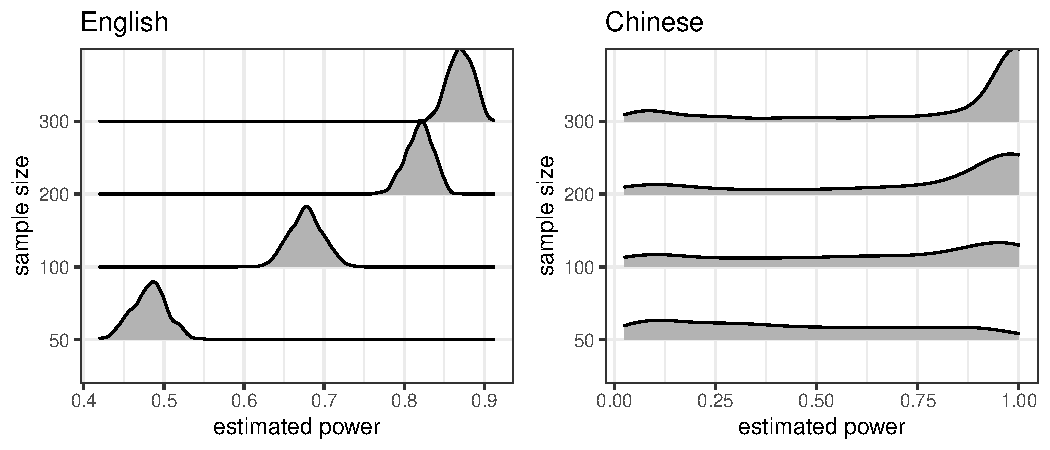
\includegraphics[width=\maxwidth]{figures/fig-unnamed-chunk-11-1} 

}


\end{knitrout}
\caption{Estimated statistical power using simulation for the English and Chinese relative clause data. Each power distribution is generated by simulating data repeatedly from an assumed effect size of $0.12~(SE: 0.05)$ log ms for English, and an assumed effect size of $-0.07~(0.05)$ log ms for Chinese. All other parameters (the variance components, and correlation) are assumed to be point values. The uncertainty in the power calculation stems from the uncertainty about the assumed effect size (the fixed effects slope), which represents the mean difference in reading time between the two relative clause types, and the uncertainty due to the variance components (the random effects). The bigger spread in the power estimates in Chinese comes from the fact that the data that the power analysis is based on were much noisier than in English (for example, in Table \ref{table:coefficients}, compare the residual standard deviations in Chinese vs.\ English: 0.52 vs.\ 0.36).}\label{fig:powerEN}
\end{figure}



%\caption{Estimated statistical power using simulation for the English and Chinese relative clause data. Each power distribution is generated by simulating data repeatedly from an assumed effect size of $0.12~(SE: 0.05)$ log ms for English, and an assumed effect size of $-0.07~(0.05)$ log ms for Chinese. All other parameters (the variance components, and correlation) are assumed to be point values. The uncertainty in the power calculation therefore reflects the uncertainty about the parameter of interest, the slope, which represents the mean difference in reading time between the two relative clause types.}\label{fig:powerEN}
%\end{figure}

\subsubsection{Results of the prospective power analyses}

Figure \ref{fig:powerEN} shows the distribution of power for sample sizes 50, 100, 200, and 300 participants and 16 items given the parameter estimates from the English Experiment 1 of \citet{grodner}, and the Chinese experiment from \citet{gibsonwu}. The bigger spread in power estimates for Chinese compared to English come from the fact that the Chinese data are much noisier (e.g., the estimated residual standard deviation in Chinese is 1.5 times larger than in English). It is clear from this plot that if we want to be reasonably sure that we have at least 80\% power, we will need at least 300 participants for this design. The original studies had sample sizes 42 and 37 \citep[][respectively]{grodner,gibsonwu}; these are severely underpowered studies. 

Thus, if planning future studies on English and Chinese, and even if one optimistically assumes that the true effect sizes are as those observed in the above two studies, the sample sizes needed to detect the effects with statistical power at approximately 80\% would be much larger than the sample sizes commonly used in such experiments.  A crucial point to keep in mind is that even with the larger sample size, the uncertainty about the power achieved---which comes from the uncertainty about the effect size---will remain. Despite this uncertainty, a larger-sample study would be a huge improvement over these two small-sample experiments.

Notice that in the above power analyses, only the uncertainty of the fixed effect predictor was taken into account, not the uncertainty associated with the variance components and correlation. If one were to take all that uncertainty into account, the power distribution would become even wider (even more uncertain). Incidentally, one can carry out a Bayesian version of a power analysis using Bayes factors, with similar results; see \citet{vasishth2021sample} for detailed discussion and example code.

In summary, despite the uncertainties inherent in power analysis, it is nevertheless a useful tool for planning sample sizes when one is committed to working within the frequentist null hypothesis testing paradigm. Even if one ends up running a small-sample study due to time or resource limitations, such power analyses can be useful for understanding how strong one's conclusions can be once the data come in. If one has no choice but to report a low-powered study's findings in a paper, then the claims have to be tempered accordingly (I illustrate later what such a tempered claim would look like). 


\section{AFTER THE DATA ARE COLLECTED}

Once the data are in, the first step should be to visualize the data and only then to carry out the statistical analysis. The visualization serves two important purposes. 

First, a boxplot or the like will reveal any extreme or potentially influential values. The mean can be extremely sensitive to extreme values, making a non-significant difference come out significant. An example is the \citet{gibsonwu} data: if we remove just two extreme data points from the data-set consisting of 547 data points, the effect becomes non-significant. The \citet{gibsonwu} paper reported this one effect as significant; just plotting the data before analyzing can prevent such erroneous reporting.\footnote{Researchers often use automated trimming procedures to remove potentially influential data points; this kind of automated data deletion is not something any statistician would do. Moreover, this automated procedure is not applied consistently even by the same research group. For example, \citet{grodner} deleted extreme values, but \citet{gibsonwu} kept the extreme values that were the sole reason for the significant effect.} 

Second, individual differences in the effect of interest should be visualized to get a sense of whether random slopes should included in the model. Often, such a visualization already makes it clear what the random effects structure of the linear mixed model should look like. Formal model comparison methods exist, but these are all completely focused on statistical significance testing. As discussed above, NHST makes no sense at all unless statistical power is high, and high statistical power is a luxury we rarely enjoy in linguistics (see section \ref{before}).  

\subsection{Visualize data before analyzing it}

Figure \ref{fig:boxplot} shows a boxplot for the English and Chinese data. It is quite striking that the variability in one condition is larger than in the other: in English, the object relative condition has larger variance, and in Chinese, it is the subject relative condition. What useful information do these plots deliver? Here are some insights from Figure \ref{fig:boxplot}.

\begin{enumerate}
\item The difference between relative clause types in English and Chinese might have to do with differences in the variance between the two conditions rather than (just) the difference in means. This heterogeneity in variance can have important consequences for statistical inference, especially when---as \citet{grodner} and  \citet{gibsonwu} did---t-tests or repeated measures ANOVA are carried out \citep{SchadEtAlAggregation2022}. Another possibility that the figure raises is that both the English and Chinese data might be generated not from a single distribution but from a hierarchical finite mixture distribution, such as a mixture of lognormals \citep{VasishthChopinRyderNicenboimCogSci2017}.
\item Even if one ignores the difference in variance between the two conditions, the extreme values could unduly influence the mean difference. As I show below, in Chinese the statistically significant effect (object relatives easier to process than subject relatives) that was reported in \citet{gibsonwu}  is determined by only two extreme data points in subject relatives,  out of a total of 547 data points.
\end{enumerate}


\begin{figure}[!htbp]
\centering
\begin{knitrout}
\definecolor{shadecolor}{rgb}{0.969, 0.969, 0.969}\color{fgcolor}

{\centering 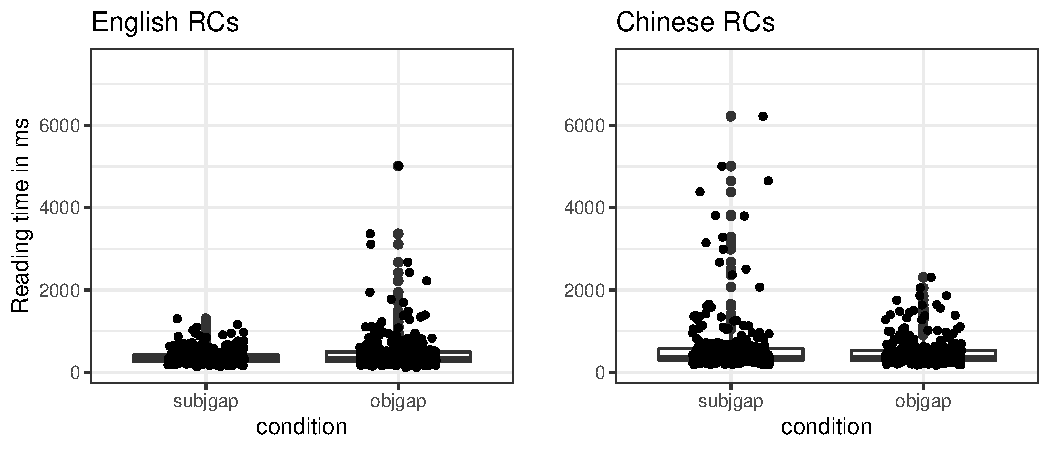
\includegraphics[width=\maxwidth]{figures/fig-unnamed-chunk-13-1} 

}


\end{knitrout}
\caption{Boxplots showing the distribution of the Grodner and Gibson (2005) Experiment 1 data on English subject and object relative clauses (left) and the Gibson and Wu (2013) data on Chinese relative clauses. Shown are reading times (in ms) by condition at the critical region (the relative clause verb).}\label{fig:boxplot}
\end{figure}

\begin{figure}[!htbp]
\centering
\begin{knitrout}
\definecolor{shadecolor}{rgb}{0.969, 0.969, 0.969}\color{fgcolor}

{\centering 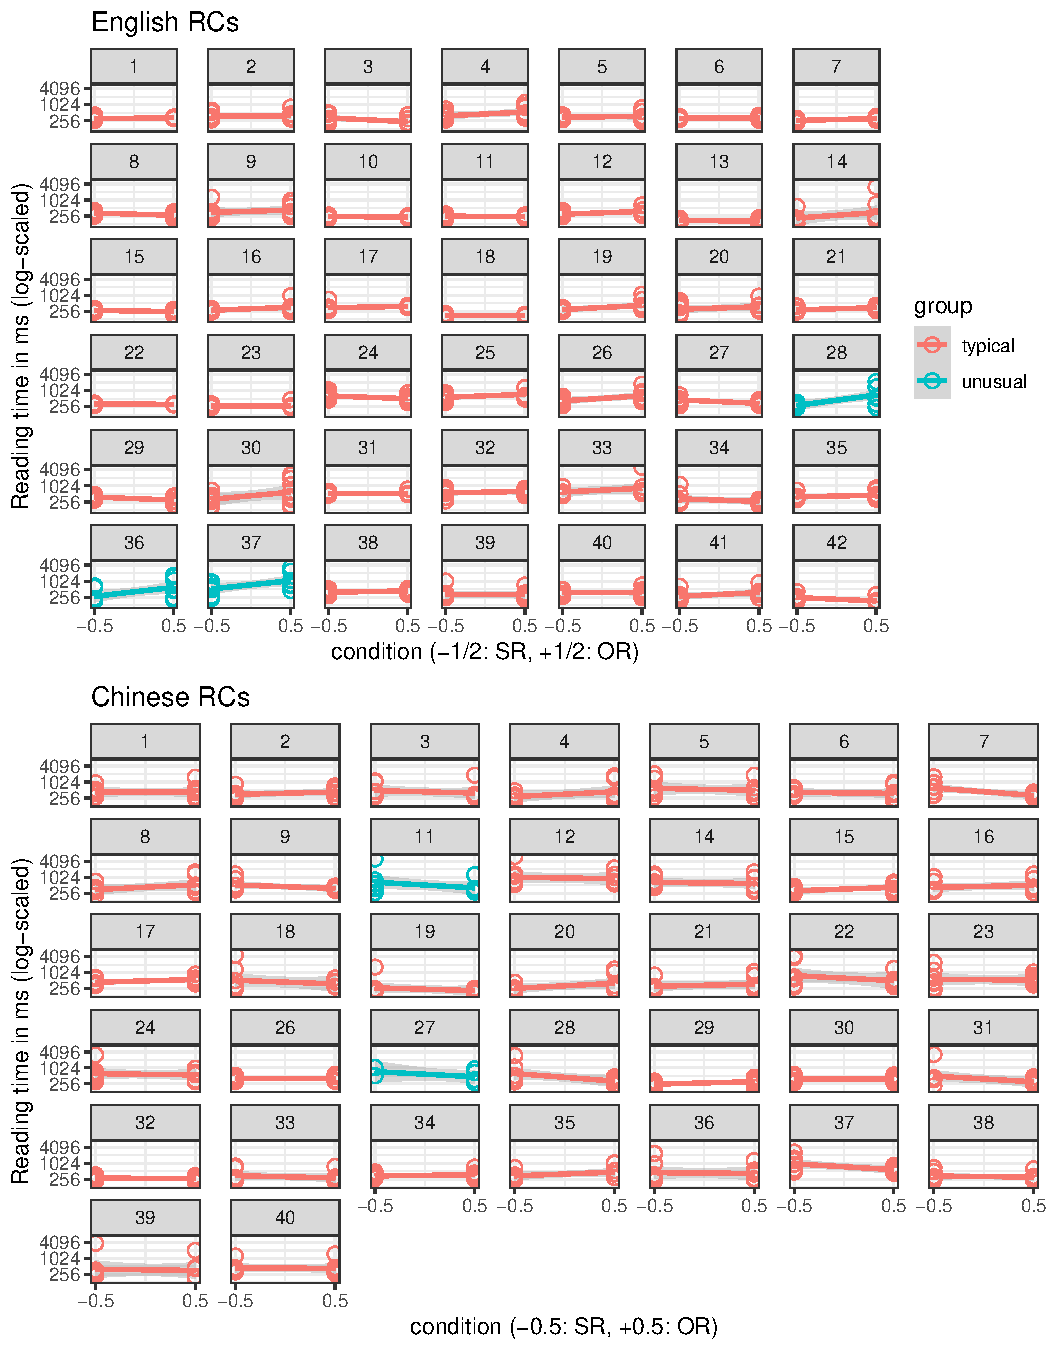
\includegraphics[width=\maxwidth]{figures/fig-unnamed-chunk-14-1} 

}


\end{knitrout}
\caption{A so-called xy-plot showing the distribution of the Grodner and Gibson (2005) Experiment 1 data on English subject and object relative clauses. Shown are log reading times by condition and by subject at the critical region (the relative clause verb). The participants with unusual responses are marked.}\label{fig:xyplot}
\end{figure}

The by-participant individual differences in the relative clause effect in English and Chinese are shown in Figure \ref{fig:xyplot}. These individual-level plots are not the shrunken estimates from the linear mixed models \citep{lme4new}, but rather use the data from each subject independently \citep[from the so-called no-pooling model, ][]{gelmanhill07,VasishthEtAlFreq2019,NicenboimEtAlBayes2019}. What do we learn from this plot?



\begin{enumerate}
\item In the English data, participants 28, 36, and 37 show the largest relative clause effects (0.9, 0.77, 0.71 log ms) compared to the other participants and compared to the mean of 0.12 log ms. On the millisecond scale, these estimates amount to a relative clause effect of 413, 319, and 543 ms, respectively. These values are 10 times larger than the average effect estimated from the linear mixed model (48 ms).
\item In the Chinese data, participant 27 has only two observations for subject relatives (7 or 8 data points are expected)! There is no explanation in \citet{gibsonwu} as to what causes this data loss.  Moreover, participant 11 has an unusually large relative clause effect, which seems to be driven by one extreme value (5006 ms reading time). This extreme value suggests that the effect of a few data points could have a dramatic impact on the statistical inference; this turns out to be the case. As I show below, if we log-transform the data, thereby reducing the impact of these extreme values, the conclusions from the data change radically.
\end{enumerate}

Apart from the above descriptive observations, these plots show considerable variation between participants, suggesting that by-particiant intercepts and slopes will probably be needed in the models. One could draw similar by item plots (omitted here to conserve space).

These figures are only relevant for the reading time data discussed here; due to space limitations, visualizations for different types of data can't be shown here. Examples of good-quality data visualizations are discussed in \citet{wilke}.

\subsection{Statistical inference}



Drawing inferences from the data requires that we specify a statistical model; deciding what an appropriate model for one's data is a subjective step. Even with seemingly simple statistical tests like the t-test,  much can go wrong if the model assumptions are not met. For example, in the one-sample t-test, violating the normality and independence assumptions will lead to invalid inferences from hypothesis tests. It is not unheard of for researchers to fit a t-test to binary data; this amounts to assuming that a Normal distribution is generating 0's and 1's; the appropriate distributional assumption would be a Bernoulli. Statistical software generally assumes that the researcher knows what they are doing and return no warning if the model assumptions are not met, so it is easy to go wrong if one treats statistical tests like automated procedures. For examples of incorrect uses of the t-test, see \citet{NicenboimRoettgeretal,VasishthEtAlFreq2019}. With linear mixed models (LMMs) fit to reading time data, violations of the normality assumption  can dramatically change the inferences we draw from the data and model. For example, in the Chinese data, if we fit the LMM to raw reading times (using the normal likelihood), then the effect comes out significant (t=-2.15); but if we remove the two extreme values in the subject relative conditions (see Figure \ref{fig:boxplot}), the t-value suddenly becomes non-significant (t=-1.76). The log-transformed analysis shown in Table \ref{table:coefficients} is unaffected by the extreme values because the log-transform downweights the two influential values.

We already saw in Table \ref{table:coefficients} what the estimates from a frequentist linear mixed model were for the English and Chinese data. If one were doing a hypothesis test using these frequentist model estimates, the standard conclusion would be that we have clear evidence for the English RC effect but not for Chinese. As we saw earlier, both conclusions would be misleading because of the danger of Type M error arising from underpowered studies.

In this section, I discuss a more nuanced way to work with such data sets. I focus on statistical inference using Bayesian hierarchical (linear mixed) models, and on two different ways of thinking about inference: estimation and hypothesis testing. The Bayesian approach is chosen here because--as I demonstrate below--it is more conservative and more flexible than standard NHST, and directly answers the research question itself (instead of rejecting a straw-man null hypothesis). Bayesian modeling also allows us to focus on quantifying the uncertainty regarding the effect of interest, instead of talking about hard binary distinctions like ``effect present/absent''.

\subsubsection{Bayesian hierarchical models}

Over the last decade or so, it has become relatively easy to fit Bayesian hierarchical (aka linear mixed) models using the programming language Stan \citep{rstan2141,carpenter2017stan}. Standard linear mixed models that linguists are used to fitting with the package \texttt{lme4} can now easily be fit using the front-end to Stan, \texttt{brms} \citep{brms}, which uses a very similar syntax.

The real barrier to using Bayesian models in research is not the mathematical or computational complexity but rather the change in perspective that is needed.

\paragraph{Some important ideas in Bayesian methodology}
In frequentist modeling, the data are random and the parameters are fixed, unknown point values. This means that the statistical inferences are based on data that we \textit{didn't} collect, and the statistical test (the t-test, the Chi-squared test, the F-score) quantifies evidence in terms of what \textit{could} have happened  hypothetically in the data assuming that some null hypothesis is true; the focus is not on the research hypothesis, but on how improbable the test statistic is in some imaginary, counterfactual world of infinite replications, given the null hypothesis. Frequentist null hypothesis significance testing doesn't tell us anything directly about the research hypothesis of interest \citep{pvals}; it only tells us what the evidence against the null is. In this sense, although NHST answers a question, it answers the wrong one.

By contrast, in the Bayesian framework, the data are considered to be fixed---you get what you get.\footnote{One can of course think about the consequences of what would happen under hypothetical repeated sampling even in the Bayesian context; in other words, we can ask ourselves what would happen if the data were random as well. See \citet{SchadEtAlWorkflow,SchadEtAlBF,vasishth2021sample} for detailed discussion.} In Bayes, it is the parameters that are random variables; parameters have probability distributions associated with them. Thinking about parameters as random variables has far-reaching implications: now we no longer talk about ``the'' relative clause effect (object minus subject relative clause processing difference) as if it's some invariant, unknown point value like 50 ms ``out there in nature'' (the reader will probably agree that it would be absurd to think about an effect as an invariant point value, but that is in fact the assumption in frequentist modeling). 
In Bayes we talk about the relative clause effect as a probability distribution. As a hypothetical example, we might believe \citep[based on prior data or theory or computational modeling; see][for how such prior information can be derived]{ohagan2006uncertain,NicenboimEtAlBayes2019} that, in self-paced reading data, the RC effect might be $Normal(\mu=50,\sigma=10)$ on the millisecond scale. This kind of statement asserts that we believe a priori (before the data from our experiment come in) that we are 95\% certain that the true value of the RC effect lies between 30 and 70 ms; the range [30,70] ms is often called a 95\% credible interval. This kind of prior knowledge/belief can then be included in the Bayesian linear mixed model to compute something called the posterior distribution of the RC effect, which gives the updated probability distribution of the RC effect after seeing the data. In other words, a critical advantage of the Bayesian paradigm we have the opportunity to formally build on prior knowledge.

Users of frequentist methods are not accustomed to thinking about and utilizing prior knowledge in data analysis, but it is standard practice in areas like medicine \citep{cochrane} to derive a quantitative summary of what is known so far, and to use that knowledge in future analyses \citep{spiegelhalter1994bayesian}. Such evidence synthesis has examples in psycholinguistics as well \citep{VasishthetalPLoSOne2013,mahowald2016meta,JaegerEngelmannVasishth2017,NicenboimRoettgeretal,NicenboimPreactivation2019,BuerkiEtAl2020,cox2022bayesian}. These kinds of meta-analyses can be very helpful in deriving prior distributions for future studies \citep{NicenboimEtAlBayes2019,VasishthEngelmann2020}.

The end-product of a Bayesian analysis is a probability distribution on the parameter (more precisely, the joint distribution of the parameters in the model); all the inferences about the research problem are made based directly on this information, not via the properties of imaginary replications of the data as in the frequentist approach. A concrete example will help.


\paragraph{A Bayesian analysis of the relative clause data}
Suppose that we re-run the linear mixed models discussed above; this time, we use the Bayesian framework. Here is the formal statement of the linear mixed model for both English and Chinese:

\begin{equation*} \label{eq:mainmodel}
rt_{ij} \sim LogNormal(\alpha + u_{0i} + w_{0j} + (\beta + u_{1i} + w_{1j}) \times so_{ij}, \sigma)
\end{equation*}

\noindent
where

\begin{equation*}\label{eq:jointpriordistLM}
\begin{pmatrix}
  u_0 \\
  u_1 \\
\end{pmatrix}
\sim
\mathcal{N} \left(
\begin{pmatrix}
  0 \\
  0 \\
\end{pmatrix},
\Sigma_{u}
\right),
\quad
\begin{pmatrix}
  w_0 \\
  w_1 \\
\end{pmatrix}
\sim
\mathcal{N}\left(
\begin{pmatrix}
  0 \\
  0 \\
\end{pmatrix},
\Sigma_{w}
\right)
\end{equation*}


\begin{equation*}\label{eq:covmatLM}
\Sigma_u
=
\begin{pmatrix}
\sigma _{u0}^2  & \rho _{u}\sigma _{u0}\sigma _{u1}\\
\rho _{u}\sigma _{u0}\sigma _{u1}    & \sigma _{u1}^2\\
\end{pmatrix}
\quad
\Sigma _w
=
\begin{pmatrix}
\sigma _{w0}^2  & \rho _{w}\sigma _{w0}\sigma _{w1}\\
\rho _{w}\sigma _{w0}\sigma _{w1}    & \sigma _{w1}^2\\
\end{pmatrix}
\end{equation*}

The \texttt{lme4} syntax for this model is:

\begin{verbatim}
lmer(log(rt) ~ so + (1+so|subj) + (1+so|item),dat)
\end{verbatim}

There are nine parameters in the model ($\alpha, \beta, \sigma_{u0}, \sigma_{u1}, \rho_u, \sigma_{w0}, \sigma_{w1}, \rho_w,\sigma$), and each parameter gets a prior distribution defined for it. Below, I define so-called regularizing priors for the parameters. 
\begin{marginnote}[]
\entry{Regularizing priors}{Regularization here means that implausible values of parameters are a priori ruled out. For example, in the frequentist model fit with \texttt{lme4}, one often sees a $+1$ or $-1$ correlation between varying intercepts and varying slopes, and/or estimates of 0 for variance components; these estimates signal a convergence failure in the \texttt{lmer} function because it implies a degenerate variance-covariance matrix \citep{pinheirobates}. This kind of convergence problem cannot occur in a Bayesian model when a regularizing prior (the LKJ prior shown below) is used on the correlation parameters \citep[of course, other convergence problems can occur but these can generally be resolved easily through methods like reparameterization or tuning the sampling algorithm; see ][for discussion]{NicenboimEtAlBayes2019}.}
\end{marginnote}

%A detailed justification for the priors used here is in \citet{SchadEtAlWorkflow}. For now it suffices to say that the prior distributions below for each of the parameters are well-motivated and very reasonable for the present research problem.

\begin{align*}
\alpha \sim& Normal(6,0.6)\\
\beta \sim& Normal(0,0.1)\\
\sigma_u, \sigma_w, \sigma \sim& Normal(0,0.5) \text{ where } \sigma_u>0\\
\rho_u, \rho_w \sim&  LKJ(2)\\
\end{align*}

The prior on the intercept $\alpha$ implies that the mean reading time can range from 122 to 1339 ms with probability 0.95. The prior on the  $\beta$ parameter implies that the RC effect can range from -81 to 81 ms with probability 0.95. This is a mildly informative prior; what this prior expresses is agnosticism about the sign of the RC effect, but also assumes that the effect is not likely to be very large. For an empirically based justification for such a mildly informative prior, see chapter 6 of \citet{NicenboimEtAlBayes2019}.

The standard deviations have truncated standard normal distributions as priors (truncated at 0 because standard deviations can't be negative); and the correlations have a so-called LKJ prior whose parameter, 2, downweights extreme correlations like $\pm 1$.













\paragraph{Results of the Bayesian analysis: Using estimation}


The posterior distributions of the relative clause effect for English and Chinese are shown in Figure \ref{fig:posteriors}. These posteriors directly answer our research questions for English and Chinese.  The estimates of the English relative clause effect are 35 ms, 95\% credible interval [2, 69] ms, and for Chinese,
-24 ms, [-66, 17] ms.

It is possible to draw our conclusions using just these estimates and their uncertainties  \citep{kruschke2010believe,kruschke2018bayesian}.
It is clear that the posterior distributions are consistent with the qualitative claim that object relatives will be harder in English and easier in Chinese compared to the respective baseline condition; however, the 95\% credible intervals shows that there is quite a lot of variability possible in the estimates. This high variability, or low precision of the estimate, is highly informative because it is an indication that we have relatively sparse data (a detail that we have already independently established with the power analysis earlier). Due to this low precision, no strong conclusions can be drawn about these effects from these data.

Now, if we want to go further and find out whether there is evidence for an RC effect in English and Chinese, i.e., if we want to make a discovery claim, we will have to do a formal hypothesis test: we will need to compute the Bayes factor  \citep{kass1995bayes}.

\begin{figure}
\centering
\begin{knitrout}
\definecolor{shadecolor}{rgb}{0.969, 0.969, 0.969}\color{fgcolor}

{\centering 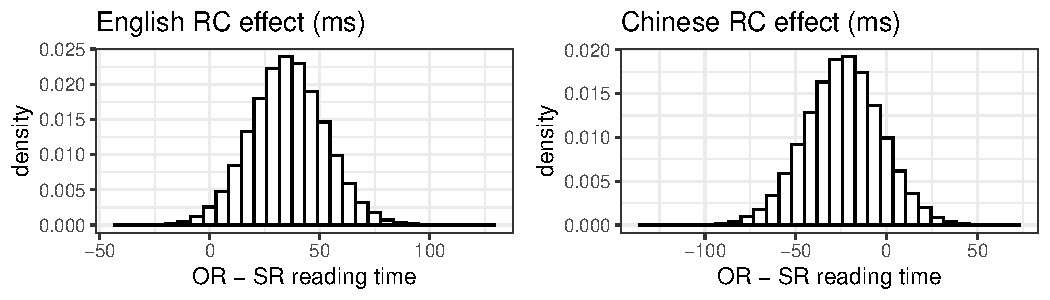
\includegraphics[width=\maxwidth]{figures/fig-unnamed-chunk-17-1} 

}


\end{knitrout}
\caption{The posterior distributions of the relative clause effect (object relative minus subject relative) in milliseconds at the critical region (the relative clause verb in English, the head noun in Chinese). These posterior distributions give us estimates of plausible values of this effect, given the Bayesian linear mixed models and the data at hand.}\label{fig:posteriors}
\end{figure}

\paragraph{Results of the Bayesian analysis: Using Bayes factors for hypothesis testing}

In essence, the Bayes factor compares the likelihood (more precisely, the marginal likelihood) of the baseline model (the so-called null model) against the likelihood based on some alternative model.
The null model could be that the parameter $\beta$, which represents the difference between the two RC types, is 0 log ms, and the alternative could be that $\beta$ is $Normal(\mu=0,\sigma=0.1)$  on the log ms scale. A powerful property of the Bayes factor is that the null and alternative models can be \textit{any} competing models \citep[e.g.,][]{rouder2021there}; one is not restricted to assuming a simple point value null hypothesis. For example, for English, one could compare a null model that assumes that the effect is a priori Normal(0,0.01) on the log ms scale (this corresponds to the 95\% credible interval  [-8,8] on the ms scale) with an alternative model that the effect is, say, Normal(0.02,0.01) in the English data (I illustrate the use of such a null hypothesis below).

The end-result of a Bayes factor analysis is the \textit{relative} likelihood of the two models being compared, presented  as a ratio. For example, when comparing a null model with the alternative, if the ratio is $3$, this means that the null model is three times more likely than the alternative, given the prior on the parameter of interest. The order in which the model comparison is done determines how the Bayes factor is interpreted; for example, if we were comparing the alternative with the null, then the Bayes factor mentioned above would be $\frac{1}{3}$. For this reason, when reporting Bayes factors, one usually signals the order in which the comparison was done: with the null model marked as 0, and the alternative as 1, we would write $BF_{01} = 3$ or $BF_{10}=\frac{1}{3}$. Generally, strong evidence in favor of the null or alternative is considered to be a Bayes factor larger than 10 \citep[this follows from a suggested scale in][]{jeffreys1998theory}. Thus, a Bayes factor analysis either gives us evidence for the alternative, evidence for the null, or an inconclusive result. 

Here, it is extremely important to understand that it makes little sense to report a single Bayes factor for a particular analysis; a so-called sensitivity analysis should be done using a range of priors on the target parameter to compute the Bayes factor \citep{SchadEtAlBF}. Such a sensitivity analysis is necessary because the Bayes factor can change depending on the prior specification \citep{lee2014bayesian}; accordingly, to interpret the Bayes factor one needs to understand what the prior distribution implies about our belief about that parameter.  An example of a sensitivity analysis will help here.

I will compute Bayes factors with three different priors on the $\beta$ parameter. The names used for the priors below are adapted from \citet{spiegelhalter1994bayesian} and \citet{Gelman14}.

\begin{enumerate}
\item The mildly informative Normal(0,0.1) prior mentioned above; here the null hypothesis is that $\beta=0$;
\item An agnostic or uninformative prior, Normal(0,1), that allows a wide range of possible values ranging from -948 ms to 948 ms; here, too, the null hypothesis is that $\beta=0$;
%\item A more liberal agnostic prior, Cauchy(0,1), that allows an even wider range of possible values ranging from minus infinity to plus infinity; here, as above, the null hypothesis is that $\beta=0$;\footnote{I include the Cauchy prior because some researchers, primarily in psychology  \citep{morey2015package}, recommend that Bayes factors be computed with a so-called `default' prior; this is usually a Cauchy distribution \citep{johnson1995continuous}. The Cauchy prior allows essentially any value for the RC effect between minus infinity and plus infinity; this is obviously completely unrealistic. As I show below, this kind of prior is usually a bad idea at least in psycholinguistic applications as it will heavily bias the hypothesis test in favor of the null hypothesis. The use of such a prior will lead to biased inferences from the Bayes factor (although the posteriors will be largely unaffected).}
\item An enthusiastic prior (one for English and another for Chinese) that represents a prior belief that is consistent with the theoretical claims discussed in \citet{grodner} and \citet{gibsonwu}. For English, the prior assumes a small but positive effect, Normal(0.02,0.01) (this assumes a 95\% credible interval from 0 ms to 16 ms), and for Chinese a small but negative effect, Normal(-0.02,0.01) (this assumes a 95\% credible interval from -16 ms to 0 ms). I will use two alternative null hypotheses:
\begin{enumerate}
\item  The null is that $\beta = 0$.
\item As an illustration of a null hypothesis that doesn't have a point value, I use Normal(0,0.01); this null hypothesis asserts that the null hypothesis is that the effect is near zero ms (ranging from -8 ms to 8 ms), but not necessarily exactly 0 ms.
\end{enumerate}
\end{enumerate}

The priors for $\beta$ are summarized below:

\begin{align*}
\beta  \sim& \begin{cases}
      Normal(0,0.1) & \text{Mildly informative prior}\\
      Normal(0,1) & \text{Agnostic/uninformative prior}\\
%      Cauchy(0,1) & \text{Agnostic prior 2}\\
      Normal(0.02,0.01) & \text{Informative (enthusiastic) prior (English)}\\
      Normal(-0.02,0.01) & \text{Informative (enthusiastic) prior (Chinese)}\\
    \end{cases}    \\
\end{align*}


\begin{table}[htp]
\tabcolsep7.5pt
\caption{The Bayes factor analysis under four different sets of priors, and posterior estimates the RC effect in English and Chinese.}\label{tab:bfsummary}
\begin{center}
\begin{tabular}{@{}l|l|l|l|c|c@{}}
 & Null & Alternative & $BF_{01}$ & Posterior mean and 95\% CrI \\
\hline
English  & $\beta=0$  & $\beta \sim Normal(0,0.1)$      &   4.55    &    35 [2, 69]   \\
        & $\beta=0$      &  $\beta \sim  Normal(0,1)$     &     0.95     &   45 [8, 85]  \\
%        & $\beta=0$      &  $\beta \sim  Cauchy(0,1)$     &     round(bfEN2,2)     &   round(mean(RC_EN2)) [round(quantile(RC_EN2,prob=0.025)), round(quantile(RC_EN2,prob=0.975))]  \\
        & $\beta = 0$      &  $\beta \sim  Normal(0.02,0.01)$     &     2.44     &   8 [2, 15]  \\
        & $\beta \sim Normal(0,0.01)$      &  $\beta \sim  Normal(0.02,0.01)$     &     2.19     &   8 [2, 15]  \\
\hline
Chinese  & $\beta=0$ &   $\beta \sim Normal(0,0.1)$      &   0.95    &    -24 [-66, 17]   \\
         & $\beta=0$   &   $\beta \sim  Normal(0,1)$     &     0.13     &   -31 [-80, 16]  \\
%         & $\beta=0$   &   $\beta \sim  Cauchy(0,1)$     &     round(bfCN2,2)     &   round(mean(RC_CN2)) [round(quantile(RC_CN2,prob=0.025)), round(quantile(RC_CN2,prob=0.975))]  \\
       & $\beta = 0$      &  $\beta \sim  Normal(-0.02,0.01)$     &     1.53     &   -9 [-18, -1]  \\
       & $\beta \sim Normal(0,0.01)$      &  $\beta \sim  Normal(-0.02,0.01)$     &     1.5     &   -9 [-18, -1]  \\
\hline
\end{tabular}
\end{center}
\end{table}

The results of the Bayes factor analysis are shown in Table \ref{tab:bfsummary}.
What does this Bayes factor analysis show? First, notice that regardless of which set of priors we choose, the evidence for the RC effect is at most 4.5 in English and not at all convincing for Chinese. So, the evidence for the RC effect is not particularly strong for either language. Second, notice that the more informative prior Normal(0,0.1) pushes the posterior closer to zero, and the informative prior in English, Normal(0.02,0.01) pushes the posterior towards the mean for this prior distribution; a similar pattern is seen in the analysis of the Chinese data. This is a general characteristic of Bayesian analysis: the posterior is a compromise between the prior and the likelihood. The more informative the prior, the more influence it has in determining the posterior. Third, notice that the mere fact that zero is or is not included in the 95\% credible interval does not tell us whether we have evidence for the RC effect; only the Bayes factor can tell us whether we have evidence for an effect (and we don't). Fourth, notice that whenever the prior is uninformative (here, Normal(0,1)), the Bayes factor is unduly biased in favor of the null hypothesis; this is one important reason why one should never use only an uninformative prior in a Bayes factor analysis \citep[cf. the advice in articles like][to compute Bayes factors using so-called `default' priors that are uninformative]{wagenmakers2018bayesian2}. Finally, one could imagine computing Bayes factors under other priors (for example, adversarial priors that express a competing theoretical prediction than the ones discussed here) if there is good reason to do this. The great advantage of the Bayes factor lies in its flexibility in allowing us to investigate the evidence for our hypothesis of interest (expressed as the prior on $\beta$) relative to some appropriate null hypothesis (we are no longer restricted to a point null like $\beta=0$ as in  frequentist NHST).

\begin{marginnote}[]
\entry{Sensitivity analysis}{In Bayesian data analysis, and Bayes factor analyses in particular, fitting a model with a range of alternative priors (particularly on the target parameter, here $\beta$) is very helpful in understand the impact of the prior on the posterior. This kind of analysis also makes it possible to investigate the data from different a priori theoretical positions.}
\end{marginnote}

Thus, the overall conclusion from the Bayes factor analysis would be that neither the English not the Chinese data furnish decisive evidence for a relative clause effect. Contrast this with the published conclusions in \citet{grodner} and \citet{gibsonwu}: in both papers, overly strong claims are made for the relative clause effect in the two languages. Given the low power that 40 participants yield for these designs, the Bayes factor analysis is much more nuanced and realistic than the simplistic analysis based on p-values.

%The Bayes factor is more conservative in delivering evidence than the p-value because the Bayes factor computes the likelihoods of the competing models by taking the uncertainty of the parameters into account' by contrast, the frequentist likelihood ratio test (ANOVA) uses a point-value, the maximumum likelihood estimate (MLE), as a proxy for the alternative hypothesis. If the MLE is biased (e.g., due to Type M error), then the conclusion will be biased, as we saw in the above examples.
It is generally the case that the Bayes factor will furnish a more realistic picture than frequentist NHST of what we learned from the data, regardless of whether we use estimation to draw inferences, or carry out explicit hypothesis testing.  
%Some researchers \citep[e.g.,][]{dienes2018four,van2021bayes} claim that Bayes factors can provide decisive evidence even in low-power studies; as I demonstrate in   \citet{vasishth2021sample}, this isn't generally true.
%In low-precision (underpowered) studies, Type M error can also lead to over-enthusiastic Bayes factors.

\section{THE ELEPHANT IN THE ROOM: HOW TO EXPRESS UNCERTAINTY AND STILL GET PUBLISHED?}

Analyzing data as suggested in this article means that we need to be willing to express uncertainty about the conclusions. Two practical problems that arise are the following: (i) Often, due to logistical or financial reasons, it may be impossible to run a properly powered study; how can one proceed in this situation? (ii) Journals generally tend to reject papers that do not make a decisive claim; wouldn't expressing uncertainty about the result lead to non-publishable results?

Regarding the first point, it is true that most studies will be similar to the \citet{grodner} and \citet{gibsonwu} studies in  being underpowered. But, as I tried to show in this article, such underpowered studies are useful and informative preliminary studies that future researchers can build on, either in a meta-analysis or for planning follow-up studies.  Of course, when possible, one should try to run as high-powered a study as one can, but if one has limited time and/or money, some data is still better than no data at all.

Regarding the standards that journals impose on papers, reviewers and editors will have to reflect on the fact that statistical analysis will usually only get us so far; those looking for certainty in statistics will be disappointed. The replication crisis should have made this clear to everyone \citep{open2015estimating}. In psycholinguistics, we are seeing the consequences of these artificial constraints imposed by journals: Type M errors will be published preferentially \citep[e.g.,][]{levy2013expectation}, non-significant results will be presented as significant through misleading analyses using aggregated data or ignoring model assumptions \citep[e.g.,][]{hsiao03,gibsonwu}, ignoring the MinF$'$ value and declaring significance anyway \citep[e.g.,][]{vandykemcelree06,fedorenko2006nature}, or repeated null results will be incorrectly argued for using severely underpowered designs \citep[e.g.,][]{vasishthlewisLanguage05}.  The alternative is to openly accept the uncertainty inherent in data \citep{VasishthGelman2021}. My own experience has has been that it is usually possible to publish underpowered studies in mainstream journals without overstating the claims \citep[e.g.,][]{NicenboimEtAlCogSci2018,VasishthMertzenJaegerGelman2018,JaegerMertzenVanDykeVasishth2019,NicenboimPreactivation2019,ALV2019,LissonEtAl2021}. 

\begin{comment}
Regardless of whether frequentist or Bayesian methods are adopted,
experimentally oriented linguistics will also benefit greatly if a  culture of cumulative science is actively fostered. As \citet{kruschke2018bayesian} and many others \citep[e.g.,][]{cumming2014new} have pointed out, a focus on estimation, uncertainty quantification, and evidence accumulation through meta-analysis will advance our understanding of phenomena much more robustly than is presently the case. A prerequisite for creating such a culture of cumulative science is that code and data be available to the reader when a paper is published. Currently, it is not normal to provide such information, and there is significant resistance to data release \citep{wicherts2006poor}. For example, \citet{LaurinavichyuteVasishth2021} investigated 57 articles that were  published in the \textit{Journal of Memory and Language} after the journal instituted a mandatory data (and code) release policy in 2019; surprisingly, 10 out of 57 articles did not release any data at all despite this being a prerequisite for publication in the journal. Even when the data are provided, the published analyses are often not reproducible; for example, \citet{LaurinavichyuteVasishth2021} found that the analyses in only about 30\% of the 47 articles that did release data were reproducible, where reproducibility is defined as bitwise reproducibility \citep{national2019reproducibility}, i.e., we should obtain identical numbers to those published in the original paper. This kind of reproducibility problem adds further uncertainty to the empirical base. It is probably possible to do much better, especially given modern tools for literate programming \citep{knuth1984literate} like Jupyter (https://jupyter.org/) and R Markdown \citep{xie2018r}.
\end{comment}

\begin{summary}[SUMMARY POINTS]
\begin{enumerate}
\item Frequentist null hypothesis significance testing is only meaningful when power is high.
\item Simulating data before conducting an experiment is a very important component of the analytical principle; simulation tells us what we can in principle learn from our experiment design.
%\item Simulating data from the model after collecting the data is also a very valuable way to understand what the model predicts.
\item Knowledge will advance better in the field if the focus is on reporting estimates and their uncertainties, without necessarily carrying out the usual, largely artificial hypothesis tests. This is likely to result in a much better quantitative understanding of the phenomenon being studied, and evidence synthesis (meta-analysis) can then be used to build on previous work.
\item To establish whether an effect exists,  a formal model comparison with a baseline model is necessary. The Bayes factor is the most conservative, informative, and flexible way to carry out such a hypothesis test.
%\item Crucial to a cumulative experimental science is transparency: open data and code, and reproducible workflows are critical for robust scientific progress
\end{enumerate}
\end{summary}


\section{OPEN DATA AND CODE STATEMENT}

Reproducible code associated with this paper is available from  https://vasishth.github.io/ANRVasishth/.

%Disclosure
\section*{DISCLOSURE STATEMENT}
The author is not aware of any affiliations, memberships, funding, or financial holdings that
might be perceived as affecting the objectivity of this review. 

% Acknowledgements
\section*{ACKNOWLEDGMENTS}

This work was funded by the Deutsche Forschungsgemeinschaft (DFG, German Research Foundation), project number 317633480, SFB 1287 (2021-2025). 


\bibliographystyle{ar-style1} 
\bibliography{/Users/shravanvasishth/Dropbox/Bibliography/bibcleaned.bib}

\end{document}

